\begin{figure*}[ht]
\begin{subfigure}{.5\textwidth}
  \centering
  % include second image
  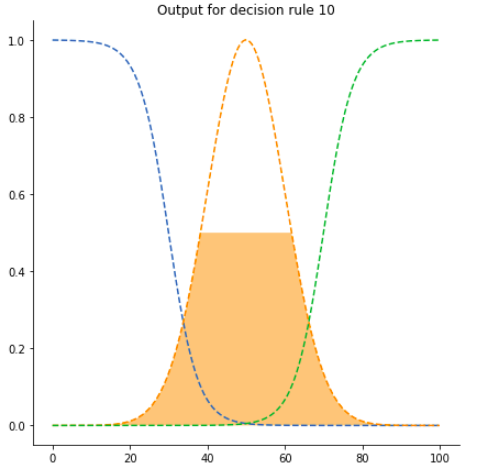
\includegraphics[width=.8\linewidth]{figures/second/min1.png}  
  \caption{Output for decision rule 10 with the T-norm minimum.}
  \label{fig:2min1}
\end{subfigure}
\begin{subfigure}{.5\textwidth}
  \centering
  % include second image
  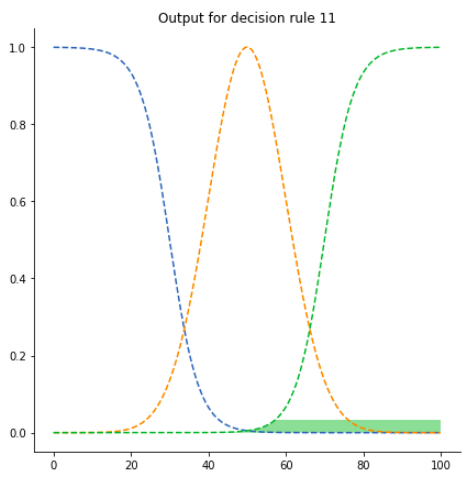
\includegraphics[width=.8\linewidth]{figures/second/min2.png}  
  \caption{Output for decision rule 11 with the T-norm minimum.}
  \label{fig:2min2}
\end{subfigure}
\begin{subfigure}{.5\textwidth}
  \centering
  % include second image
  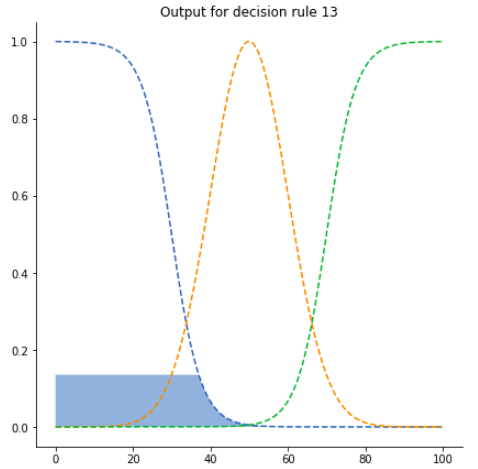
\includegraphics[width=.8\linewidth]{figures/second/min3.png}  
  \caption{Output for decision rule 13 with the T-norm minimum.}
  \label{fig:2min3}
\end{subfigure}
\begin{subfigure}{.5\textwidth}
  \centering
  % include second image
  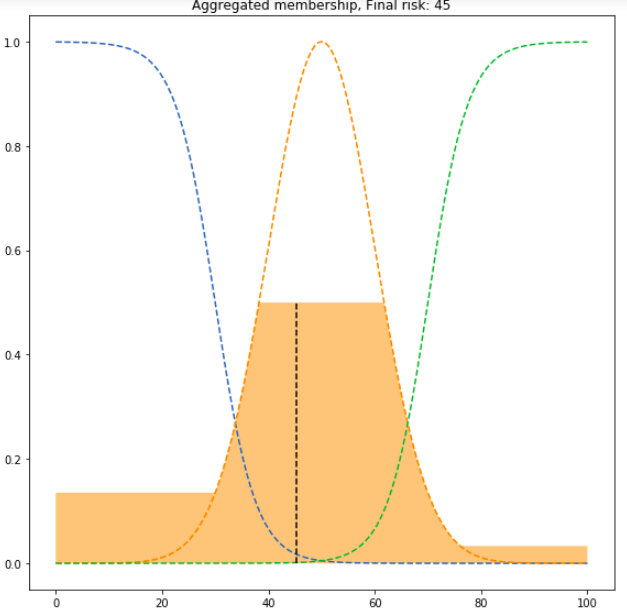
\includegraphics[width=.8\linewidth]{figures/second/min-centroid.png}  
  \caption{Final aggregation result with the centroid method for defuzzification.}
  \label{fig:2min-centroid}
\end{subfigure}
\begin{subfigure}{.5\textwidth}
  \centering
  % include second image
  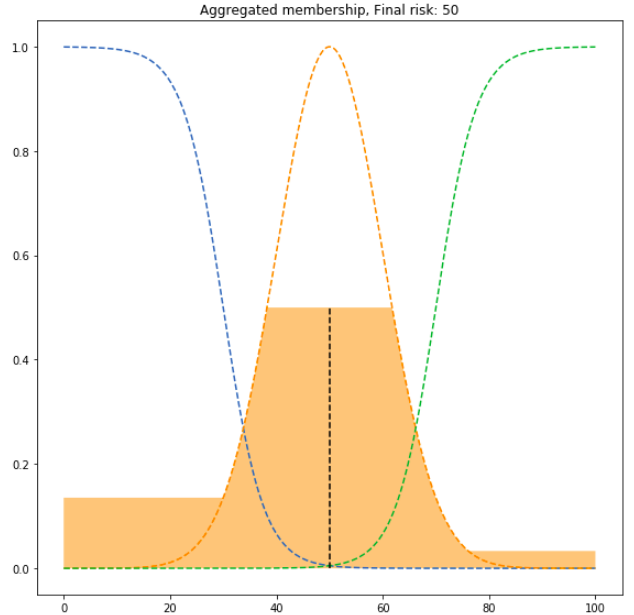
\includegraphics[width=.8\linewidth]{figures/second/min-mom.png}  
  \caption{Final aggregation result with the mean of maximum method for defuzzification.}
  \label{fig:2min-mom}
\end{subfigure}
\begin{subfigure}{.5\textwidth}
  \centering
  % include second image
  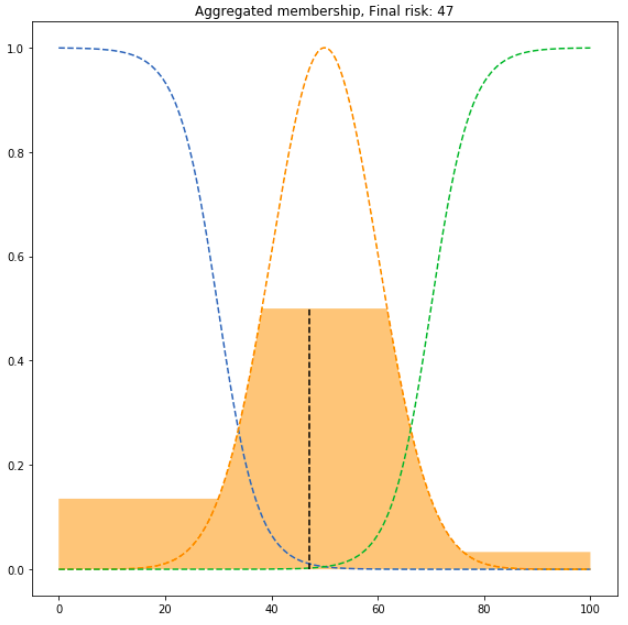
\includegraphics[width=.8\linewidth]{figures/second/min-bisector.png}  
  \caption{Final aggregation result with the bisector method for defuzzification.}
  \label{fig:2min-bisector}
\end{subfigure}
\caption{Results for test case 2 using the T-norm minimum.}
\label{fig:testcase2min}
\end{figure*}

\begin{figure*}[ht]
\begin{subfigure}{.5\textwidth}
  \centering
  % include second image
  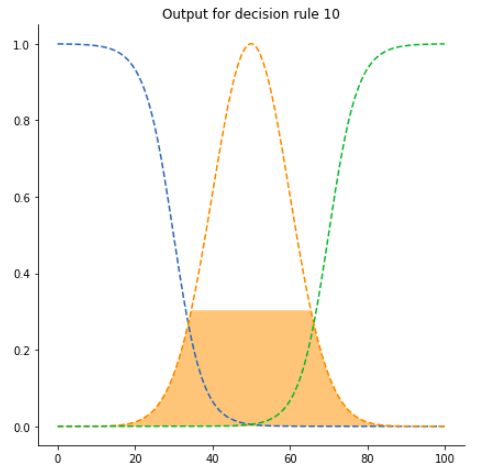
\includegraphics[width=.8\linewidth]{figures/second/prod1.png}  
  \caption{Output for decision rule 10 with the T-norm product.}
  \label{fig:2prod1}
\end{subfigure}
\begin{subfigure}{.5\textwidth}
  \centering
  % include second image
  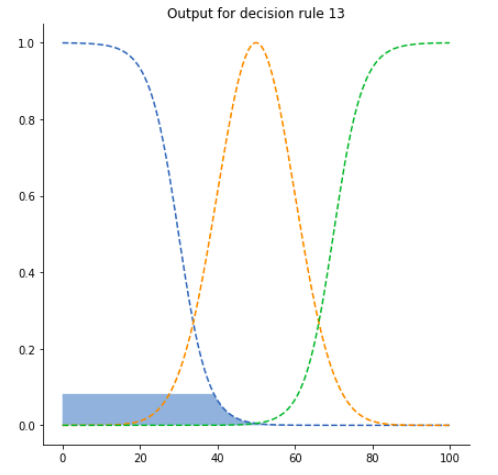
\includegraphics[width=.8\linewidth]{figures/second/prod2.png}  
  \caption{Output for decision rule 13 with the T-norm product.}
  \label{fig:2prod2}
\end{subfigure}
\begin{subfigure}{.5\textwidth}
  \centering
  % include second image
  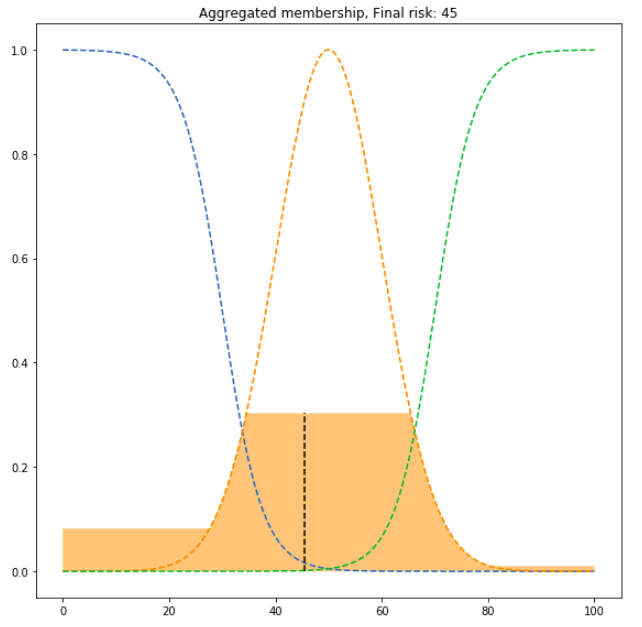
\includegraphics[width=.8\linewidth]{figures/second/prod-centroid.png}  
  \caption{Final aggregation result with the centroid method for defuzzification.}
  \label{fig:2prod-centroid}
\end{subfigure}
\begin{subfigure}{.5\textwidth}
  \centering
  % include second image
  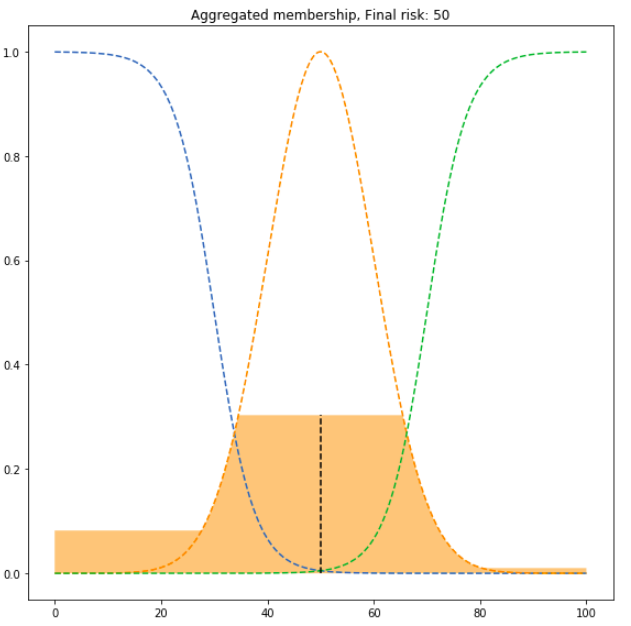
\includegraphics[width=.8\linewidth]{figures/second/prod-mom.png}  
  \caption{Final aggregation result with the mean of maximum method for defuzzification.}
  \label{fig:2prod-mom}
\end{subfigure}
\begin{subfigure}{.5\textwidth}
  \centering
  % include second image
  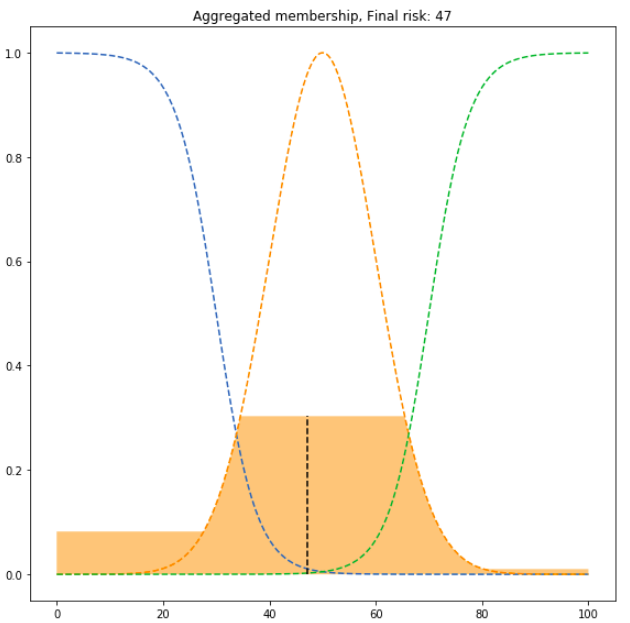
\includegraphics[width=.8\linewidth]{figures/second/prod-bisector.png}  
  \caption{Final aggregation result with the bisector method for defuzzification.}
  \label{fig:2prod-bisector}
\end{subfigure}
\caption{Results for test case 2 using the T-norm product.}
\label{fig:testcase2prod}
\end{figure*}
